\let\negmedspace\undefined
\let\negthickspace\undefined
\documentclass[journal]{IEEEtran}
\usepackage[a5paper, margin=10mm, onecolumn]{geometry}
%\usepackage{lmodern} % Ensure lmodern is loaded for pdflatex
\usepackage{tfrupee} % Include tfrupee package

\setlength{\headheight}{1cm} % Set the height of the header box
\setlength{\headsep}{0mm}     % Set the distance between the header box and the top of the text

\usepackage{gvv-book}
\usepackage{gvv}
\usepackage{cite}
\usepackage{amsmath,amssymb,amsfonts,amsthm}
\usepackage{algorithmic}
\usepackage{graphicx}
\usepackage{textcomp}
\usepackage{xcolor}
\usepackage{txfonts}
\usepackage{listings}
\usepackage{enumitem}
\usepackage{mathtools}
\usepackage{gensymb}
\usepackage{comment}
%\usepackage{multiclo}
\usepackage[breaklinks=true]{hyperref}
\usepackage{tkz-euclide} 
\usepackage{listings}
% \usepackage{gvv} 
\graphicspath{ {./figs/} }

\begin{document}


\title{
ASSIGNMENT 6: GATE 2020 \\
BM:BIOMEDICAL ENGINEERING}
\author{AI25BTECH11010 - Dhanush Kumar}
\maketitle
\renewcommand{\thefigure}{\theenumi}
\renewcommand{\thetable}{\theenumi}

\begin{enumerate}

\item Rajiv Gandhi Khel Ratna Award was conferred \underline{\hspace{2cm}}. Mary Kom, a six-time world champion in boxing, recently in a ceremony \underline{\hspace{2cm}}. the Rashtrapati Bhawan (the President’s official residence) in New Delhi.  


	\hfill(GATE BM 2020)
\begin{multicols}{2}
\begin{enumerate}
  \item with, at
  \item on, in
  \item on, at
  \item to, at
\end{enumerate}
\end{multicols}

\item Despite a string of poor performances, the chances of K. L. Rahul’s selection in the team are \underline{\hspace{2cm}}.  

	\hfill(GATE BM 2020)
\begin{multicols}{2}
\begin{enumerate}
  \item slim
  \item bright
  \item obvious
  \item uncertain
\end{enumerate}
\end{multicols}


\item Select the word that fits the analogy:  

Cover : Uncover :: Associate : \underline{\hspace{2cm}}.  

\hfill(GATE BM 2020)
\begin{multicols}{2}
\begin{enumerate}
  \item Unassociate
  \item Inassociate
  \item Misassociate
  \item Dissociate
\end{enumerate}
\end{multicols}

\item Hit by floods, the kharif (summer sown) crops in various parts of the country have been affected. Officials believe that the loss in production of the kharif crops can be recovered in the output of the rabi (winter sown) crops so that the country can achieve its food-grain production target of 291 million tons in the crop year 2019–20 (July–June). They are hopeful that good rains in July–August will help the soil retain moisture for a longer period, helping winter sown crops such as wheat and pulses during the November–February period.  

Which of the following statements can be inferred from the given passage?  


\hfill(GATE BM 2020)
\begin{enumerate}
  \item Officials declared that the food-grain production target will be met due to good rains.
  \item Officials want the food-grain production target to be met by the November–February period.
  \item Officials feel that the food-grain production target cannot be met due to floods.
  \item Officials hope that the food-grain production target will be met due to a good rabi produce.
\end{enumerate}


\item The difference between the sum of the first $2n$ natural numbers and the sum of the first $n$ odd natural numbers is  \underline{\hspace{2cm}}. 

	\hfill(GATE BM 2020)
\begin{multicols}{4}
\begin{enumerate}
  \item $n^2 - n$
  \item $n^2 + n$
  \item $2n^2 - n$
  \item $2n^2 + n$
\end{enumerate}
\end{multicols}


\item Repo rate is the rate at which Reserve Bank of India (RBI) lends commercial banks, and reverse repo rate is the rate at which RBI borrows money from commercial banks.  

Which of the following statements can be inferred from the above passage?  


\hfill(GATE BM 2020)
\begin{enumerate}
  \item Increase in repo rate will increase cost of borrowing and decrease lending by commercial banks.
  \item Increase in repo rate will decrease cost of borrowing and increase lending by commercial banks.
  \item Increase in repo rate will decrease cost of borrowing and decrease lending by commercial banks.
  \item Decrease in repo rate will decrease cost of borrowing and increase lending by commercial banks.
\end{enumerate}



\item P, Q, R, S, T, U, V, and W are seated around a circular table.  


	\hfill(GATE BM 2020)
\begin{enumerate}
\item S is seated opposite to W.  
\item U is seated at the second place to the right of R.  
\item T is seated at the third place to the left of R.  
\item V is a neighbour of S.  
\end{enumerate}

Which of the following must be true?  


\hfill(GATE BM 2020)
\begin{enumerate}
  \item P is a neighbour of R.
  \item Q is a neighbour of R.
  \item P is not seated opposite to Q.
  \item R is the left neighbour of S.
\end{enumerate}



\item The distance between Delhi and Agra is 233 km. A car $P$ started travelling from Delhi to Agra and another car $Q$ started from Agra to Delhi along the same road 1 hour after the car $P$ started. The two cars crossed each other 75 minutes after the car $Q$ started. Both cars were travelling at constant speed. The speed of car $P$ was 10 km/hr more than the speed of car $Q$. How many kilometers the car $Q$ had travelled when the cars crossed each other?  


	\hfill(GATE BM 2020)
\begin{multicols}{4}
\begin{enumerate}
  \item 66.6
  \item 75.2
  \item 88.2
  \item 116.5
\end{enumerate}
\end{multicols}


\item For a matrix $M = [m_{ij}],\ i,j = 1,2,3,4$, the diagonal elements are all zero and $m_{ij} = -m_{ji}$.  
The minimum number of elements required to fully specify the matrix is \underline{\hspace{2cm}}.  

\hfill(GATE BM 2020)
\begin{multicols}{4}
\begin{enumerate}
  \item 6
  \item 8
  \item 10
  \item 16
\end{enumerate}
\end{multicols}


\item The profit shares of two companies P and Q are shown in the figure. If the two companies 
have invested a fixed and equal amount every year, then the ratio of the total revenue of 
company P to the total revenue of company Q, during 2013--2018 is \underline{\hspace{2cm}}.



    \begin{figure}[H]
    \centering
	    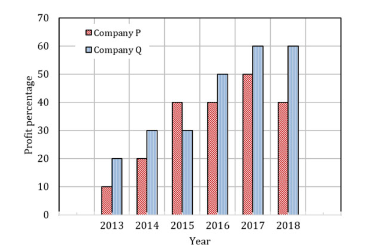
\includegraphics[width=0.6\textwidth]{Screenshot_2025_0822_151008.png}
\caption{}
    \label{fig:Q10}
\end{figure}

\hfill(GATE BM 2020)
\begin{multicols}{2}
\begin{enumerate}
\item 15 : 17
\item 16 : 17
\item 17 : 15
\item 17 : 16
\end{enumerate}
\end{multicols}


\item $m_1$ and $m_2$ are the roots of the characteristic equation of a linear second order 
physical system. Match the nature of the roots with the natural response of the system. \\[6pt]
\begin{table}[H]
	\centering\normalsize
\begin{tabular}{|l|l|}
	\hline
	Nature of roots &Systen respones \\\hline	
P. $m_1$ and $m_2$ are real and distinct & K. Critically damped \\\hline
Q. $m_1$ and $m_2$ are equal & L. Overdamped \\\hline
R. $m_1$ and $m_2$ are complex & M. Underdamped \\
	\hline
\end{tabular}
\caption{}                                        
\label{tab:Q11}                                   
\end{table}


\hfill(GATE BM 2020)
\begin{multicols}{2}
\begin{enumerate}
\item P-L, Q-M, R-K
\item P-M, Q-L, R-K
\item P-L, Q-K, R-M
\item P-M, Q-K, R-L
\end{enumerate}
\end{multicols}


\item A person is sitting in a chair with feet on the ground. While rising up on his feet, the 
kinematic motion \textbf{NOT} occurring is:


\hfill(GATE BM 2020)
\begin{multicols}{2}
\begin{enumerate}
\item Hip extension
\item Plantar flexion
\item Hip flexion
\item Knee extension
\end{enumerate}
\end{multicols}

\item The equipment that measures elasticity of blood vessel \textit{in vivo} is:


	\hfill(GATE BM 2020)
\begin{enumerate}
\item Rheometer
\item Dimension analyser
\item Thermomechanical analyser
\item Dynamic mechanical analyser
\end{enumerate}

\item Biomaterials with shape memory effects are NOT used in:


	\hfill(GATE BM 2020)
\begin{enumerate}
\item Intracranial aneurysm clips
\item Arterial blood vessel closure devices
\item Orthopedic total joint replacements
\item Orthodontic dental wires
\end{enumerate}



\item The MRI scanner parameter of long $T_{rep}$ or short $T_{echo}$ will generate a \underline{\hspace{2cm}}
contrast image.

\hfill(GATE BM 2020)
\begin{multicols}{2}
\begin{enumerate}
\item Proton Density--weighted
\item T2--weighted
\item T1--weighted
\item T2*--weighted
\end{enumerate}
\end{multicols}


\item In diagnostic X-ray imaging, the following is NOT a part of primary EM radiation 
interaction in soft tissue:


\hfill(GATE BM 2020)
\begin{enumerate}
\item Photoelectric effect
\item Characteristic radiation production
\item Compton scattering
\item Pair-production
\end{enumerate}


\item A 5 MHz ultrasound pulse is used to image a tumor at a depth of 2 cm in a soft tissue. 
It takes time $t$ for the reflected echo from the tumor to come back to the receiver. Instead, 
if a 2.5 MHz wave is used, how long will it take for the echo from the same tumor to arrive 
at the receiver?


\hfill(GATE BM 2020)
\begin{multicols}{4}
\begin{enumerate}
\item $t/2$
\item $t$
\item $2t$
\item $4t$
\end{enumerate}
\end{multicols}


\item $X(s)$ is the Laplace transform of a signal $x(t)$. The Laplace transform of 
$\dfrac{dx(t)}{dt}$ assuming $x(0)=0$, is:

\hfill(GATE BM 2020)
\begin{multicols}{4}
\begin{enumerate}
\item $sX(s)$
\item $\dfrac{X(s)}{s}$
\item $tX(s)$
\item $\dfrac{dx}{ds}$
\item $\dfrac{1}{s}\dfrac{dx}{ds}$
\end{enumerate}
\end{multicols}


\item Which of the following are odd functions? \\[4pt]
P: $\sin(t)$ \\
Q: $\cos(t)$ \\
R: $\sin(t)+\cos(t)$ \\
S: $\sin(t)\cos(t)$


\hfill(GATE BM 2020)
\begin{multicols}{4}
\begin{enumerate}
\item Q and S
\item P and Q
\item P and R
\item P and S
\end{enumerate}
\end{multicols}

\item State-space model of a system is given as:
\[
	\vec{\dot{X}} = 
\myvec{
a & 2 \\
0 & b
}X +
\myvec{
1 \\
0
}U,
\quad
vec{Y}= \myvec{1 & 0}X
\]

The conditions for the system to be controllable are


\hfill(GATE BM 2020)
\begin{multicols}{4}
\begin{enumerate}
    \item $a=0, \; b \ne 0$
    \item $a \ne 0, \; b=0$
    \item $a \ne 0, \; b \ne 0$
    \item $a=0, \; b=0$
\end{enumerate}
\end{multicols}

\item In microprocessor systems with memory mapped I/O, which of the following is true?



	\hfill(GATE BM 2020)
\begin{enumerate}
    \item Only I/O devices with internal memory can be interfaced.
    \item I/O devices can be accessed using IN and OUT instructions.
    \item Each I/O device can be addressed as a memory location.
    \item Arithmetic and logic operations cannot be directly performed with the I/O data.
\end{enumerate}

\item The number of electrodes used in recording standard 12-lead Electrocardiogram (ECG) is


	\hfill(GATE BM 2020)
\begin{multicols}{4}
\begin{enumerate}
    \item 13
    \item 10
    \item 11
    \item 12
\end{enumerate}
\end{multicols}

\item Which of the following is \textbf{NOT} a part of knee joint?


	\hfill(GATE BM 2020)
\begin{multicols}{4}
\begin{enumerate}
    \item Patella
    \item Tibia
    \item Femur
    \item Fibula
\end{enumerate}
\end{multicols}

\item During a routine stethoscope examination at the left midclavicular-5th intercostal space, murmurs were noted between first and second heart sound. The possible abnormality among the following could be


	\hfill(GATE BM 2020)

\begin{enumerate}
    \item Aortic stenosis
    \item Mitral regurgitation
    \item Mitral stenosis
    \item Aortic regurgitation
\end{enumerate}


\item The thin filament of a muscle fiber is comprised of



	\hfill(GATE BM 2020)
\begin{enumerate}
    \item Troponin, Tropomyosin, Actin
    \item Troponin, Tropomyosin, Titin
    \item Tropomyosin, Titin, Actin
    \item Actin, Myosin, Troponin
\end{enumerate}


\item The value of the integral evaluated over the contour $C: |z|=3/2$ is
\[
\frac{1}{2\pi j}\oint_C \frac{z}{(z-1)(z-2)}\,dz
\]


\hfill(GATE BM 2020)
\item The eigenvalues of a $3\times 3$ non-singular matrix $P$ are $1,2,3$. The trace of matrix $P^{-1}$ (rounded off to two decimal places) is \underline{\hspace{2cm}}


	\hfill(GATE BM 2020)
\item The following recursion relation, when started from a finite positive non-zero value, converges to \underline{\hspace{2cm}}
\[
x_{n+1} = \frac{1}{2}\left(x_n + \frac{1}{x_n}\right)
\]

\hfill(GATE BM 2020)

\item In a nuclear imaging system, sodium iodide (NaI) crystals are used to detect gamma rays of 120 keV. The percentage (\%) of gamma-rays that will pass through 1 cm of NaI crystal, assuming the Half-Value-Layer (HVL) of NaI as 0.2 cm, is \underline{\hspace{2cm}} (rounded off to one decimal place).

	\hfill(GATE BM 2020)

\item The distal end of an endoscope is placed at a distance of 1 mm from the gastrointestinal wall. The refractive indices of the fiber core and cladding are $1.5$ and $1.45$, respectively. The maximum field of view for the endoscope is \underline{\hspace{2cm}} degrees (rounded off to one decimal place).


	\hfill(GATE BM 2020)


\item Two inductors with the details given below are wound separately on two identical ring type ferromagnetic cores.  

\begin{table}[H]                                    
\centering\normalsize
\begin{tabular}{|c|c|c|c|}
\hline
Coil & Number of turns & Gauge of wire & Self-Inductance \\
\hline
Coil-1 & N & G & L\_1 \\
\hline
Coil-2 & 2N & G/2 & L\_2 \\
\hline
\end{tabular}
	\caption{}
	\label{tab:Q21}
\end{table}
The ratio $L_2/L_1$ is \underline{\hspace{2cm}}


\hfill(GATE BM 2020)
\item Two dyes X and Y having concentrations in the ratio $0.25$ in identical cuvettes were subjected to absorption measurements in a spectrophotometer. The estimated ratio of their absorbance is $0.5$. The ratio of their molar extinction coefficients is \underline{\hspace{2cm}}


	\hfill(GATE BM 2020)
\item Hydrolysis of one ATP molecule provides an energy of \underline{\hspace{2cm}} kilo calories (rounded off to one decimal place).


	\hfill(GATE BM 2020)
\item An 830 nm laser Doppler flow meter probe is oriented at an angle of $60^\circ$ to the flow axis. If the average flow velocity is 3 cm/s, the magnitude of Doppler shift frequency (kHz) is \underline{\hspace{2cm}} (rounded off to one decimal place).


	\hfill(GATE BM 2020)

\item A 100 mA single current pulse from a pulse generator is used for artificial pacing of heart at the right ventricle. If the delivered energy does not exceed the fibrillation threshold of 300 $\mu$J, the safe duration of the pulse that could be applied to the tissue mass having an impedance of 500 $\Omega$ is \underline{\hspace{2cm}} $\mu$s.

	\hfill(GATE BM 2020)

\item  The resting potential of a mammalian nerve cell is $-80$ mV. A certain drug administered to the body changes the intracellular K$^+$ concentration from 150 mmol/L to 55 mmol/L. The nearest value of cell membrane potential after the drug administration, assuming that the external equilibrium of K$^+$ does not get changed during the event, is 

\begin{itemize}
    \item[] (Gas constant $= 8.315$ J/mol/K, core temperature $= 37^\circ$C and
    \item[] Faraday constant $= 96500$ C/mol)
\end{itemize}


\hfill(GATE BM 2020)
\begin{multicols}{4}
\begin{enumerate}
    \item $-117.7$ mV
    \item $-18.77$ mV
    \item $-53.32$ mV
    \item $-141.20$ mV
\end{enumerate}
\end{multicols}

\item  The arrangement of four resistors of equal value in the diaphragm of a physiological pressure measurement catheter is shown below. When applied pressure deforms the diaphragm, there is an increase in length of resistors R2 and R4 and a decrease in length of resistors R1 and R3. The changes in resistance value are proportional to the length of individual four resistors. Which among the configuration given below should be used to form a Wheatstone bridge circuit such that bridge output voltage is proportional to the change in resistance of individual resistors?


    \begin{figure}[H]
    \centering
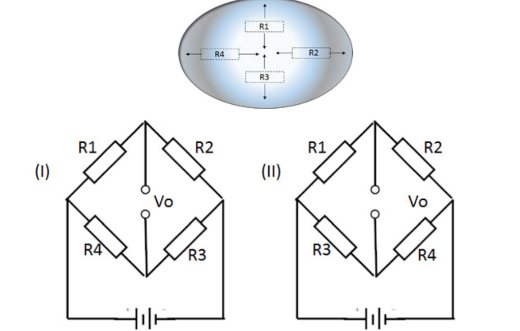
\includegraphics[width=0.6\textwidth]{Screenshot_2025_0822_155841.png}
\caption{}
    \label{fig:Q37}
\end{figure}

\hfill(GATE BM 2020)
\begin{multicols}{2}
\begin{enumerate}
    \item I only
    \item II only
    \item Neither I nor II
    \item Both I and II
\end{enumerate}
\end{multicols}

\item  For the given input voltage, $V_{in} = 10 \sin(2 \pi t)$ to the functional circuit shown below, the output signal will be

\begin{figure}[H]
	\centering                                  
	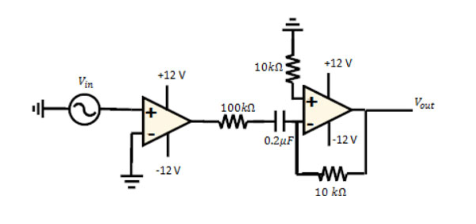
\includegraphics[width=0.6\textwidth]{Screenshot_2025_0822_155855.png}
 \caption{}
   \label{fig:Q38}                                   
\end{figure}
      
      
      \hfill(GATE BM 2020)
\begin{multicols}{2}

	 \begin{figure}[H]
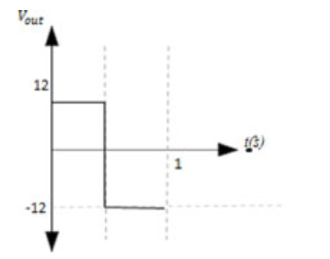
\includegraphics[width=0.45\textwidth]{Screenshot_2025_0822_155912.png}  
	 \caption*{(a)}
  \label{fig:Q38option1}
 \end{figure}
 
  \begin{figure}[H]
  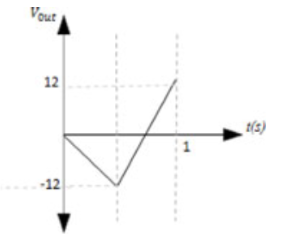
\includegraphics[width=0.45\textwidth]{Screenshot_2025_0822_155921.png} \\
        \caption*{(b)}
   \label{fig:Q38option2}
   \end{figure}
 
 \begin{figure}[H]
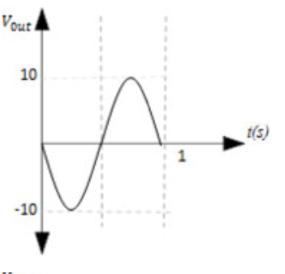
\includegraphics[width=0.45\textwidth]{Screenshot_2025_0822_155928.png} \\
       \caption*{(c)}
   \label{fig:Q38option3}
   \end{figure}

 \begin{figure}[H]
  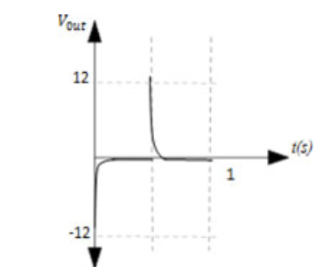
\includegraphics[width=0.45\textwidth]{Screenshot_2025_0822_155937.png} \\
         \caption*{(d)}
 \label{fig:38option4}
\end{figure}
 \end{multicols}

\item  During a non-invasive measurement of blood pressure, mean arterial pressure was observed to be 100 mm Hg. If systolic pressure is 150 mm Hg, the diastolic pressure would be


	\hfill(GATE BM 2020)
\begin{multicols}{4}
\begin{enumerate}
    \item 110 mm Hg
    \item 75 mm Hg
    \item 70 mm Hg
    \item 50 mm Hg
\end{enumerate}
\end{multicols}
	
\item Two loads are connected to AC supply mains as depicted in the figure. One load draws 10 kW whereas the other load of 10 kVA is operated at 0.6 pf lagging. To achieve an overall power factor of 0.9544 lagging, the nearest kVAr rating of the capacitor bank needed to be connected across the supply mains is equal to


    \begin{figure}[H]
    \centering
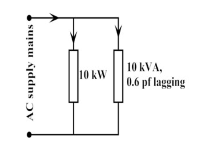
\includegraphics[width=0.6\textwidth]{Screenshot_2025_0822_162240.png}
\caption{}
    \label{fig:Q40}
\end{figure}


\hfill(GATE BM 2020)

\begin{multicols}{4}
\begin{enumerate}
\item 3
\item 5
\item 7
\item 9
\end{enumerate}
\end{multicols}

\item The nearest value of power dissipated in the $3 \, \Omega$ resistance in the circuit is


    \begin{figure}[H]
    \centering
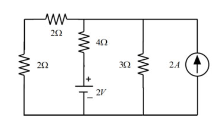
\includegraphics[width=0.6\textwidth]{Screenshot_2025_0822_162246.png}
\caption{}
    \label{fig:Q41}
\end{figure}


\hfill(GATE BM 2020)

\begin{multicols}{4}
\begin{enumerate}
\item 3 W
\item 25/3 W
\item 12 W
\item 25/12 W
\end{enumerate}
\end{multicols}

\item A second order low pass filter is being constructed by cascading two first order low pass filters with the following transfer functions

\[
H_1(j\omega) = \frac{1}{1 + j \frac{\omega}{\omega_1}}, 
\quad 
H_2(j\omega) = \frac{1}{1 + j \frac{\omega}{\omega_2}}
\]

where $\omega_1$ and $\omega_2$ are the respective 3dB cut-off frequencies.  

The undamped natural frequency $\omega_n$ of the resulting second order low pass filter is


\hfill(GATE BM 2020)
\begin{multicols}{2}
\begin{enumerate}
\item $\omega_n = \sqrt{\omega_1 \omega_2}$
\item $\omega_n = \omega_1 + \omega_2$
\item $\omega_n = \dfrac{\omega_1 \omega_2}{\omega_1 + \omega_2}$
\item $\omega_n = \sqrt{\omega_1^2 + \omega_2^2}$
\end{enumerate}
\end{multicols}

\item Match the bridge type with the application given below:


	
	\begin{table}[H]
	\centering\normalsize
\begin{tabular}{|c|l|}
\hline
\textbf{Name of the bridge} & \textbf{Application} \\
\hline
P. Maxwell bridge        & K. Measurement of Low resistance \\
Q. Kelvin double bridge  & L. Measurement of medium Q-coil inductance \\
R. Hay bridge            & M. Measurement of capacitance \\
S. Schering bridge       & N. Measurement of High Q-coil inductance \\
\hline
\end{tabular}
\caption{}                                   
\label{tab:Q43}                              
\end{table}


\hfill(GATE BM 2020)
\begin{multicols}{2}
\begin{enumerate}
\item P-L, Q-K, R-N, S-M
\item P-N, Q-K, R-L, S-M
\item P-N, Q-L, R-M, S-K
\item P-L, Q-M, R-N, S-K
\end{enumerate}
\end{multicols}


\item For a non-unity feedback system with 
\[
G(s) = \frac{12}{s(s+2)} \quad \text{and} \quad H(s) = \frac{2}{s(s+3)},
\]
the magnitude of steady-state error to a unit step-input is


\hfill(GATE BM 2020)
\begin{multicols}{4}
\begin{enumerate}
\item 0.50
\item 0.45
\item 0.25
\item 0.20
\end{enumerate}
\end{multicols}


\item Match the Boolean expression with its minimal realization:



	\begin{table}[H]
	\centering\normalsize
\begin{tabular}{|c|l|}
\hline
\textbf{Boolean expression} & \textbf{Minimal realization} \\
\hline
P. $XYZ + \overline{X}YZ + XY\overline{Z}$ & K. $X(Y+Z)$ \\\hline
Q. $XYZ + X\overline{Y}Z + XY\overline{Z}$ & L. $X(Y+Z)$ \\\hline
R. $XY\overline{Z} + X\overline{Y}Z + \overline{X}YZ$ & M. $YZ$ \\\hline
S. $XYZ + XY\overline{Z} + X\overline{Y}Z + \overline{X}YZ$ & N. $Y(X+Z)$ \\
\hline
\end{tabular}
	\caption{}
	\label{tab:Q45}
\end{table}


\hfill(GATE BM 2020)
\begin{multicols}{2}
\begin{enumerate}
\item P-K, Q-L, R-N, S-M
\item P-L, Q-K, R-N, S-M
\item P-L, Q-K, R-M, S-K
\item P-N, Q-K, R-L, S-M
\end{enumerate}
\end{multicols}

\item The glomerulus filtration process of kidney is modeled as a flat membrane with pores of radius 1 nm and length of pore 60 nm. The viscosity of the fluid is 0.002 Pa.s. The aggregate area of the pores makes 5\% of total surface area of the membrane. The average pressure over the blood side of the membrane is 8000 Pa and on the ultrafiltrate side is 6200 Pa. The total available area of membrane is 1.5 m$^2$. The nearest value of resulting filtration rate in cm$^3$/min is


\hfill(GATE BM 2020)

\begin{multicols}{2}
\begin{enumerate}
  \item 0.14
  \item 1.40
  \item 8.43
  \item 34.7
\end{enumerate}
\end{multicols}


\item During resting state, the voltage outside the cell membrane compared to that inside the membrane is \underline{\hspace{1.5cm}}. Under such conditions, the intracellular and extracellular regions have \underline{\hspace{1.5cm}} and \underline{\hspace{1.5cm}} concentrations, respectively.



	\hfill(GATE BM 2020)
\begin{enumerate}
  \item More positive, more Potassium [K$^+$], more Sodium [Na$^+$]
  \item More negative, more Potassium [K$^+$], more Sodium [Na$^+$]
  \item More negative, more Sodium [Na$^+$], more Potassium [K$^+$]
  \item More positive, more Sodium [Na$^+$], more Potassium [K$^+$]
\end{enumerate}

\item The tensile strength of a degradable suture used for a surgical procedure in the human body shows 60\% decrease exponentially for 10 days. The tensile strength shows 80\% after 10 days and 20 days, respectively. The closest approximation (in days) for the tensile strength to decay to 20\% of its original value would be



	\hfill(GATE BM 2020)
\begin{multicols}{4}
\begin{enumerate}
  \item 26
  \item 33
  \item 43
  \item 52
\end{enumerate}
\end{multicols}


\item A 60 kg person is standing on one foot on a force plate. The ground reaction force is found to act 60 mm anterior to the ankle joint. The knee joint is 60 mm from the Trochanter Knee Ankle (TKA) line. If the weight of the foot is 18.5 kg, the closest value of \textit{magnitude} of moment acting on the ankle joint is


	\hfill(GATE BM 2020)

\begin{multicols}{4}
\begin{enumerate}
  \item 23 Nm
  \item 248 Nm
  \item 223 Nm
  \item 466 Nm
\end{enumerate}
\end{multicols}

\item The temperature of bone cement is increased from 37$^\circ$C to 87$^\circ$C during the femoral hip arthroplasty. The cement thickness is noted to be 20 mm. The stress developed due to exothermic reaction of bone cement during the polymerization process and shrinkage of the bone cement, respectively, are

\textbf{Assume that:}
\begin{itemize}
  \item bone, cement, and implant are modeled as a set of concentric cylinders
  \item no direct adhesion takes place between bone and cement
  \item temperature is uniform
\end{itemize}

Coefficient of thermal expansion of bone cement $= 90 \times 10^{-6}/^\circ$C

Young’s modulus of bone cement $= 3.5$ GPa


\hfill(GATE BM 2020)
\begin{multicols}{2}
\begin{enumerate}
  \item 15.75 MPa, 90 µm
  \item 15.75 MPa, 110 µm
  \item 6.85 MPa, 110 µm
  \item 6.85 MPa, 90 µm
\end{enumerate}
\end{multicols}


\item An object is imaged in a 1 Tesla MRI scanner and induced voltage is found to be equal to $V_0$. The expression for the magnitude of the received voltage in RF coil is given by
\[
|V| = 2 \pi \gamma M_0 (\sin \alpha) f
\]
When the patient is shifted to a 3 Tesla MRI scanner that uses the same RF coil and the slice thickness is halved, the magnitude of the induced voltage was found to be equal to $V_2$. The ratio $V_2/V_1$ is


\hfill(GATE BM 2020)
\begin{multicols}{4}
\begin{enumerate}
  \item 1.5
  \item 3.0
  \item 4.5
  \item 6.0
\end{enumerate}
\end{multicols}


\item A 3 MHz ultrasound transducer transmits a 3-cycle long pulse into a soft tissue at normal incidence to fat and liver interface. The axial resolution (mm) and the amplitude reflection coefficient at fat-liver interface, respectively, are

\[
c_{\text{tissue}} = 1500 \,\text{m/s}, \quad c_{\text{fat}} = 1450 \,\text{m/s}, \quad c_{\text{liver}} = 1570 \,\text{m/s}
\]

\[
\rho_{\text{fat}} = 920 \,\text{kg/m}^3, \quad \rho_{\text{liver}} = 1060 \,\text{kg/m}^3
\]


\hfill(GATE BM 2020)
\begin{multicols}{2}
\begin{enumerate}
  \item 0.75, 0.22
  \item 0.75, 0.12
  \item 0.5, 0.22
  \item 0.5, 0.11
\end{enumerate}
\end{multicols}


\item The forward biased current of a silicon (Si) diode is being calculated from the exponential model of the V-I characteristics. If the diode current $I_D = 1$ mA at a voltage drop $V_D = 0.7$ V, the nearest value of $I_D$ when $V_D = 0.8$ V is
\[
I = I_S \exp\left(\frac{V_D}{V_T}\right)
\]
Assume thermal voltage $V_T = 25.3$ mV for Si diode.


\hfill(GATE BM 2020)
\begin{multicols}{2}
\begin{enumerate}
  \item 0.133 mA
  \item 2 mA
  \item 7.5 mA
  \item 22 mA
\end{enumerate}
\end{multicols}


\item A continuous random variable $x$ has a probability density function given by
\[
f(x) = ce^{-|x|}, \qquad -\infty < x < \infty
\]
where $c$ is a real constant. The variance of $x$ is \underline{\hspace{2cm}} (correct up to one decimal place).


\hfill(GATE BM 2020)
\item The magnitude of the gradient of the function $f(x,y) = x^2 + y^2$ at the point (1,1) is \underline{\hspace{2cm}} (correct up to two decimal places).


	\hfill(GATE BM 2020)

\item The value of the following double integral is \underline{\hspace{3cm}} (correct up to three decimal places).
\[
\iint_R xy \, dx\,dy
\]
where $R$ is the first quadrant of the circle with center at the origin and radius of one unit. \\


\hfill(GATE BM 2020)
\item A gynaecologist recorded the blood pressure (BP) of patients as shown in the Table below. Using Regression process, the diastolic BP of a 38 year old patient (mm Hg) is \underline{\hspace{3cm}} (rounded off to two decimal places).


    \begin{figure}[H]
    \centering
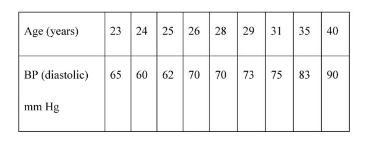
\includegraphics[width=0.6\textwidth]{Screenshot_2025_0822_171940.png}
\caption{}
    \label{fig:Q60}
\end{figure}


\hfill(GATE BM 2020)
\item A person in standing position first flexes the hip by $50^\circ$ from the initial Trochanter knee ankle (TKA) line and then flexes knee by $20^\circ$. The distance of ankle joint from the initial TKA line is \underline{\hspace{3cm}} (rounded off to nearest integer). \\
(i) The distance between hip joint and knee joint is 400 mm \\
(ii) The distance between knee joint and ankle joint is 300 mm \\


\hfill(GATE BM 2020)
\item A chest radiograph of $36 \,\text{cm} \times 48 \,\text{cm}$ is digitized. If we want to preserve details in the image to a spatial resolution of $6$ cycles/mm, the approximate image data size in MB for an 8 bit quantization is \underline{\hspace{3cm}} (rounded off to two decimal places). \\


	\hfill(GATE BM 2020)
\item The X-ray radiography scenario is shown in the figure. If the number of incident photons ($N_i$) is equal to $2 \times 10^6$ at 50 keV, the number of photons ($N_d$) that exit the tissue is \underline{\hspace{3cm}} $\times 10^6$ (rounded off to two decimal places). \\

(use linear attenuation coefficient for soft tissue and blood at 50 keV as 0.4 cm$^{-1}$ and 0.2 cm$^{-1}$, respectively).


    \begin{figure}[H]
    \centering
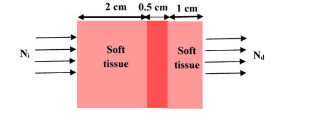
\includegraphics[width=0.6\textwidth]{Screenshot_2025_0822_165154.png}
\caption{}
    \label{fig:Q60}
\end{figure}


\hfill(GATE BM 2020)


\item The wavelength of an electron accelerated to a potential of 1 V is \underline{\hspace{3cm}} nm (rounded off to two decimal places). \\
Mass of electron = $9.11 \times 10^{-31}$ kg \\
Planck’s constant, $h = 6.63 \times 10^{-34}$ Js \\
Charge of electron = $1.6 \times 10^{-19}$ C \\


\hfill(GATE BM 2020)
\item In a permanent magnetic moving coil (PMMC) instrument having following specifications, the angular deflection of the pointer for a coil current of 100 $\mu$A will be \underline{\hspace{3cm}} degrees (rounded off to one decimal place). \\

Magnetic flux density = 1.5 Tesla \\
Torsional spring constant = $2 \times 10^{-6}$ Nm/deg \\
Cross sectional area of the coil = 2.5 cm$^2$ \\
Number of turns of the coil = 500 \\

\hfill(GATE BM 2020)

\item Arterial blood extracted from a healthy adult showed an oxygen partial pressure value of 40 mm Hg. The total oxygen content in the arterial blood measured in \%V/V is \underline{\hspace{2cm}} (rounded off to one decimal place).

\[
\text{Given:}
\]
\[
\text{Solubility of oxygen in blood} = 0.003 \, \text{ml/mm Hg/dL}
\]
\[
\text{Hemoglobin oxygen saturation} = 95\%
\]
\[
\text{Oxygen carrying capacity of Hb} = 1.34 \, \text{ml/g}
\]
\[
\text{Arterial blood hemoglobin concentration} = 15 \, \text{g/dL}
\]


\hfill(GATE BM 2020)
\item In the process of measuring blood flow from an artery using C-clamp magnetic flow probe, the voltage recorded across diametrically opposite sites of the artery is 3.75 nV. The blood flow rate through the artery is \underline{\hspace{2cm}} cm$^3$/s (rounded off to two decimal places).

\[
\text{The inner diameter of the C-clamp} = 0.5 \, \text{cm},
\]
\[
\text{The magnetic flux density} = 1.5 \times 10^{-5} \, \text{Wb/m}^2.
\]

\item A cell is injected with a current 
\[
i(t) = u(t)
\]
to produce a change in the intracellular membrane voltage 
\[
v(t).
\]
The cell-membrane is modeled as a linear system with impulse response 
\[
h(t) = A e^{-\tfrac{t}{\tau}} u(t).
\]
The cell membrane voltage output at 5 ms is \underline{\hspace{2cm}} mV.

\[
\text{Use } A = -34 \, \text{V/s}; \quad \tau = 3 \, \text{ms}.
\]



\hfill(GATE BM 2020)
\end{enumerate}

\begin{center}
	\huge{END OF QUESTION PAPER}
\end{center}
\end{document}

